\documentclass{beamer}
\usetheme{AnnArbor}
\usecolortheme{seahorse}
\input{commands_packages}
\graphicspath{{Figures/}}
\newcommand{\Col}{\text{Col}}
\usepackage{tabu, rotating, graphicx, multicol, empheq}
%\usepackage[dvipsnames]{color}
\usepackage[framemethod=TikZ]{mdframed}

\newcommand<>{\colorize}[4]{\only<#1>{#4}\only<#2>{\textcolor{#3}{#4}}}
\newcommand{\after}[2]{\colorize{1}{2-}{#1}{#2}}
\newcommand{\ago}{\after{green}{1}}
\newcommand{\go}{\textcolor{green}{1}}
\newcommand{\ono}{\textcolor{orange}{-1}}

\newcommand{\g}[1]{\textcolor{gray}{#1}}
\usepackage[euler-digits]{eulervm} 
\usetikzlibrary{decorations.pathreplacing,angles,quotes}

\begin{document}
\title{M\"obius Inversion}   
\author{Leo Selker \\ Advisor: Vin de Silva} 
\date{\today} %February 10, 2017

\frame{\titlepage} 

\section{Adding Up Integers}
\frame{\frametitle{Cumulative Sums}
We start with some sequences of numbers:

\begin{align*}
& f: 1, 1, 1, 1, \dots  && f: 2, 2, 2, 2, \dots  && f: 1, 2, 3, 4, \dots \\
& g: 1, 2, 3, 4, \dots  && g: 2, 4, 6, 8, \dots  && g: 1, 3, 6, 10, \dots
\end{align*}
\vspace{.3cm}\\

\begin{enumerate}[]
\item<2-> In each case, $g_n = f_1 + f_2 + \cdots + f_n$, a cumulative sum.\vspace{.2cm}
\item<3->\[g_n = \sum_{m \leq n} f_n\]
\end{enumerate}
}

\frame{\frametitle{Going the Other Way}
How do we get from $g$ back to $f$?\\

 

\begin{align*}
& f: 1, 1, \after{green}{1}, 1, \dots  && f: 2, 2, \after{green}{2}, 2, \dots  && f: 1, 2, \after{green}{3}, 4, \dots \\
& g: 1, \after{green}{2, 3}, 4, \dots  && g: 2, \after{green}{4, 6}, 8, \dots  && g: 1, \after{green}{3, 6}, 10, \dots
\end{align*}
\onslide<2->\[
f_n = g_n - g_{n-1}
\]
\only<3>{
\color{purple}
\begin{empheq}[box=\fbox]{align*} 
g_n - g_{n-1} &= \textcolor{blue}{f_1 + ... + f_{n-1}} + f_n\\
 &-\textcolor{blue}{f_1 + ... + f_{n-1}}
\end{empheq}
}
\only<4>{
\begin{align*}
&\text{Let }\mu(m,n) = \begin{cases}
1 & m = n\\
-1 & m = n-1\\
0 & else.
\end{cases}
& \text{Then }f_n = \sum_{m \leq n}g_m\mu(m,n).
\end{align*}
}

}
\frame{\frametitle{Another Perspective}
We consider the first five values of each sequence as a vector:
\begin{align*}
& \mathbf{f} = [1, 1, 1, 1, 1]   && \mathbf{f} = [2, 2, 2, 2, 2]  && \mathbf{f} = [\after{green}{1, 2, 3, 4}, 5] \\
& \mathbf{g} = [1, 2, 3, 4, 5]  && \mathbf{g} = [2, 4, 6, 8, 10]  && \mathbf{g} = [1, 3, 6, \after{green}{10}, 15]
\end{align*}
And we encode the adding up process in a matrix:
\[\zeta = 
\begin{bmatrix}
1 & 1 & 1 & \after{green}{1} & 1\\
0 & 1 & 1 & \after{green}{1} & 1\\
0 & 0 & 1 & \after{green}{1} & 1\\
0 & 0 & 0 & \after{green}{1} & 1\\
0 & 0 & 0 & 0 & 1\\
\end{bmatrix}
\]
Then:
\[ \mathbf{g} = \mathbf{f} \zeta\]
}
\frame{\frametitle{Inverting $\zeta$ to get $\mu$}

\begin{align*}\zeta  = 
&\begin{bmatrix}
\begin{array}{rrrrr}
1 & 1 & 1 & 1 & 1\\
0 & 1 & 1 & 1 & 1\\
0 & 0 & 1 & 1 & 1\\
0 & 0 & 0 & 1 & 1\\
0 & 0 & 0 & 0 & 1\\
\end{array}
\end{bmatrix}\hspace{1cm}
\mu =\zeta^{-1} = 
&&\begin{bmatrix}
\begin{array}{rrrrr}
1 & -1 & 0 & 0 & 0\\
0 & 1 & -1 & 0 & 0\\
0 & 0 & 1 & -1 & 0\\
0 & 0 & 0 & 1 & -1\\
0 & 0 & 0 & 0 & 1\\
\end{array}
\end{bmatrix}\\
\vspace{.5cm}\\
& g_n = \sum_{m \leq n} f_n \textcolor{gray}{\zeta(m,n)}&& f_n  = \sum_{m \leq n}g_m\mu(m,n)\\
\end{align*}
}
\frame{\frametitle{Using $\mu$ to get $\mathbf{f}$}
We said that $\mathbf{g} = \mathbf{f}\zeta$, so $\mathbf{f} = \mathbf{g}\mu$.
An example:
\begin{align*}
& \mathbf{f} = [1, 2, 3, \after{green}{4}, 5]\\
& \mathbf{g} = [1, 3, \after{blue}{6}, \after{purple}{10}, 15] 
\end{align*}
\begin{align*}
\mathbf{f}= \mathbf{g}\mu = [1, 3, \after{blue}{6}, \after{purple}{10}, 15]\begin{bmatrix}
\begin{array}{rrrrr}
1 & -1 & 0 & 0 & 0\\
0 & 1 & -1 & 0 & 0\\
0 & 0 & 1 & \after{blue}{-1} & 0\\
0 & 0 & 0 & \after{purple}{1} & -1\\
0 & 0 & 0 & 0 & 1\\
\end{array}
\end{bmatrix}
\end{align*}
\onslide<2->

\[\textcolor{green}{4} = \textcolor{blue}{(-1)6} + \textcolor{purple}{(1)10}
\]
}
\frame{\frametitle{Analogy to Calculus}
What we did looks familiar.
\begin{align*}
\mathbf{g} = \mathbf{f}\zeta &\iff \mathbf{f} = \mathbf{g} \mu \\
\vspace{.5cm}\\
g(n) = \sum_{m \leq n}f(m) &\iff f(n) = \sum_{m \leq n}g(m)\mu(m,n)\\
\vspace{.8cm}\\
\only<2->{\color{blue}``g(x) = \int_1^x f(t)dt &\color{blue}\iff f(t) = \frac{d}{dx}g(t)"}
\end{align*}

}

\frame{\frametitle{Another Dimension}
We can represent functions on $m,n$ using tables of values:
\begin{align*}
f: \begin{tabu}{c|cccc}
& & & &n\\
\hline
& \ago  & \ago & \ago & \ago\\
& \ago & \ago & \ago& \ago\\
m & \ago & \ago & \ago & \ago
\end{tabu}\hspace{1cm}
g: 
\begin{tabu}{c|cccc}
& & & & n\\
\hline
& 1  & 2 & 3 & 4\\
& 2 & 4 & 6 &10\\
m & 3 & 6 & 9 & \after{green}{12} 
\end{tabu}
\end{align*}
We have
\[
g(m,n) = \sum_{(m',n')\leq(m,n)}f(m', n'),
\]
a generalized cumulative sum.
}
\frame{\frametitle{Another Dimension}
How do we get $f$ from $g$?
\begin{align*}
f: \begin{tabu}{c|cccc}
& & & &n\\
\hline
& 1  & 1 & 1 & 1\\
& 1 & 1 & 1& 1\\
m & 1 & 1 & 1 & \ago
\end{tabu}\hspace{1cm}
g: 
\begin{tabu}{c|cccc}
& & & & n\\
\hline
& 1  & 2 & 3 & 4\\
& 2 & 4 & \colorize{1-5}{6-}{blue}{6} & \colorize{1-4}{5-}{brown}{10}\\
m & 3 & 6 & \colorize{1-3}{4-}{orange}{9} & \colorize{1-2}{3-}{purple}{12}
\end{tabu}
\end{align*}

\begin{tikzpicture}[overlay]
\only<3->{\draw[purple,thick,rounded corners] (3.3,.5) rectangle (5.3,1.83);}
\only<4->{\draw[orange,thick,rounded corners] (3.3,.5) rectangle (4.8,1.83);}
\only<5->{\draw[brown,thick,rounded corners] (3.3,.9) rectangle (5.3,1.83);}
\only<6->{\draw[blue,thick,rounded corners] (3.3,.9) rectangle (4.8,1.83);}
\end{tikzpicture}
\[
\onslide<2-> \textcolor{green}{1} = 
\onslide<3->  \textcolor{purple}{12} 
\onslide<4-> - \textcolor{orange}{9}
\onslide<5-> - \textcolor{brown}{10}
\onslide<6-> + \textcolor{blue}{6}
\]
\onslide<7->
In general (finding $\mu$ would have told us this):
\[
\textcolor{green}{f(m,n)} = \textcolor{purple}{g(m,n)} - \textcolor{orange}{g(m, n-1)} - \textcolor{brown}{g(m-1, n)} + \textcolor{blue}{g(m-1, n-1)}
\]
}

\frame{\frametitle{Two Equivalent Statements}
$X, \leq$ a partially ordered set.

\begin{mdframed}
$f(x),g(x)$ functions, then
\[
g(x) = \sum_{y \leq x}f(y) \iff f(x) = \sum_{y \leq x}g(y)\color{purple}{\mu(y,x)}
\]
\end{mdframed}
\begin{mdframed}
$\bf{f}, \bf{g}$ vectors, $\zeta$ encodes $\leq$, $\mu = \zeta^{-1}$. Then
\[
\mathbf{g} = \mathbf{f}\zeta \iff \mathbf{f} = \mathbf{g}\mu
\]
\end{mdframed}
We use the matrix $\mu$ to find the function $\mu$, and to find $f$ given $g$.
}
\frame{\frametitle{What do we know about $\zeta$ and $\mu$?}
Some facts about $\zeta$ and $\mu$:
\begin{itemize}
\item $\zeta$ is upper triangular, with ones on the main diagonal. Therefore:
\item $\zeta$ is invertible, so we can write $\mu = \zeta^{-1}$, and
\item $\mu$ will have integer values.
\end{itemize}
Often, entries of $\mu$ will be -1, 0, 1. 

}
\section{Euler's Totient}
\frame{\frametitle{Integers and Divisibility}
We now replace $\leq$ with $|$ ($a|b$ if $a$ divides $b$ without remainder).  Some functions:
\begin{align*}
& f: 1, 1, 1, 1, 1, 1, 1, 1, \dots  && f: 0, 1, 0, 0, 0, 0,0, 0,  \dots  \\
& g: 1, 2, 2, 3, 2, 4, 2, 4, \dots  && g: 0, 1, 0, 1, 0, 1, 0, 1,\dots \\
\end{align*}
\onslide<2->
The first $g$ is the number of divisors. The second indicates the even numbers.

\onslide<3->
We will construct the matrices $\zeta$ and $\mu$ for the integers up to 10, and see what it tells us about how to go back from $g$ to $f$.
}
\frame{\frametitle{Constructing $\zeta$}
\[
\zeta = \bordermatrix{
 & \g{1} & \g{2} & \g{3} & \g{4} & \g{5} & \g{6} & \g{7} & \g{8} & \g{9} & \g{10} \cr
\g{1} & \go & \go & \go & \go & \go & \go & \go & \go & \go & \go  \cr
\g{2} & 0 & \go & 0 & \go & 0 & \go & 0 & \go & 0 & \go  \cr
\g{3} & 0 & 0 & \go & 0 & 0 & \go & 0 & 0 & \go & 0  \cr
\g{4} & 0 & 0 & 0 & \go & 0 & 0 & 0 & \go & 0 & 0  \cr
\g{5} & 0 & 0 & 0 & 0 & \go & 0 & 0 & 0 & 0 & \go  \cr
\g{6} & 0 & 0 & 0 & 0 & 0 & \go & 0 & 0 & 0 & 0  \cr
\g{7} & 0 & 0 & 0 & 0 & 0 & 0 & \go & 0 & 0 & 0  \cr
\g{8} & 0 & 0 & 0 & 0 & 0 & 0 & 0 & \go & 0 & 0  \cr
\g{9} & 0 & 0 & 0 & 0 & 0 & 0 & 0 & 0 & \go & 0  \cr
\g{10}& 0 & 0 & 0 & 0 & 0 & 0 & 0 & 0 & 0 & \go  \cr
}\]
}
\frame{\frametitle{Inverting $\zeta$ to get $\mu$}
\[
\zeta = \bordermatrix{
 & \g{1} & \g{2} & \g{3} & \g{4} & \g{5} & \g{6} & \g{7} & \g{8} & \g{9} & \g{10} \cr
\g{1} & \go & \ono & \ono & 0 & \ono & \go & \ono & 0 & 0 & \go  \cr
\g{2} & 0 & \go & 0 & \ono & 0 & \ono & 0 & 0 & 0 & \ono  \cr
\g{3} & 0 & 0 & \go & 0 & 0 & \ono & 0 & 0 & 0 & 0  \cr
\g{4} & 0 & 0 & 0 & \go & 0 & 0 & 0 & \ono & 0 & 0  \cr
\g{5} & 0 & 0 & 0 & 0 & \go & 0 & 0 & 0 & 0 & \ono  \cr
\g{6} & 0 & 0 & 0 & 0 & 0 & \go & 0 & 0 & 0 & 0  \cr
\g{7} & 0 & 0 & 0 & 0 & 0 & 0 & \go & 0 & 0 & 0  \cr
\g{8} & 0 & 0 & 0 & 0 & 0 & 0 & 0 & \go & 0 & 0  \cr
\g{9} & 0 & 0 & 0 & 0 & 0 & 0 & 0 & 0 & \go & 0  \cr
\g{10}& 0 & 0 & 0 & 0 & 0 & 0 & 0 & 0 & 0 & \go  \cr
}\]
}
\frame{\frametitle{What is $\mu$?}
It turns out that
\[
\mu(a,b) = \begin{cases}
0 & a \nmid b \text{ or } \frac ba \text{ is divisible by a square}\\
(-1)^{\text{\#prime factors of }\frac ba} & else
\end{cases}
\]
}
\frame{\frametitle{What is $\mu$?}
\[
\small
\zeta = \bordermatrix{
 & \g{1} & \g{2} & \g{3} & \g{4} & \g{5} & \g{6} & \g{7} & \g{8} & \g{9} & \g{10} \cr
\g{1} & \go & \ono & \ono & 0 & \ono & \textcolor{purple}{1} & \ono & 0 & 0 & \go  \cr
\g{2} & 0 & \go & 0 & \ono & 0 & \ono & 0 & 0 & 0 & \ono  \cr
\g{3} & 0 & 0 & \go & 0 & 0 & \ono & 0 & 0 & 0 & 0  \cr
\g{4} & 0 & 0 & 0 & \go & 0 & 0 & 0 & \ono & 0 & 0  \cr
\g{5} & 0 & 0 & 0 & 0 & \go & 0 & 0 & 0 & 0 & \ono  \cr
\g{6} & 0 & 0 & 0 & 0 & 0 & \go & 0 & 0 & 0 & 0  \cr
\g{7} & 0 & 0 & 0 & 0 & 0 & 0 & \go & 0 & 0 & 0  \cr
\g{8} & 0 & 0 & 0 & 0 & 0 & 0 & 0 & \go & 0 & 0  \cr
\g{9} & 0 & 0 & 0 & 0 & 0 & 0 & 0 & 0 & \go & 0  \cr
\g{10}& 0 & 0 & 0 & 0 & 0 & 0 & 0 & 0 & 0 & \go  \cr
}\]

\[\color{purple}\mu(1,6) = (-1)^2 = 1\]

}
\frame{\frametitle{Visualizing $\mu$}
\only<1>{
\begin{align*}
& f: 1, 1, 1, \textcolor{gray}{1, 1}, 1, \textcolor{gray}{1, 1}, \dots  \\
& g: 1, 2, 2, \textcolor{gray}{3,2}, 4, \textcolor{gray}{2,4}, \dots  
\end{align*}
}
\only<2->{
\[
\mu(a,b) = \begin{cases}
0 & a \nmid b \text{ or } \frac ba \text{ is divisible by a square}\\
(-1)^{\text{\#prime factors of }\frac ba} & else
\end{cases}
\]}
Values of $f,g$ on multiples of $2, 3$:
\begin{align*}
f: \begin{tabu}{c|cccc}
&2^0 &2^1 &2^2 &2^3\\
\hline
3^0& 1  & 1 & 1 & 1\\
3^1& 1 & 1 & 1& 1\\
3^2 & 1 & 1 & 1 & \ago
\end{tabu}\hspace{1cm}
g: 
\begin{tabu}{c|cccc}
&2^0 &2^1 &2^2 &2^3\\
\hline
3^0& 1  & 2 & 3 & 4\\
3^1& 2 & 4 & \colorize{1-5}{6-}{blue}{6} & \colorize{1-4}{5-}{brown}{10}\\
3^2 & 3 & 6 & \colorize{1-3}{4-}{orange}{9} & \colorize{1-2}{3-}{purple}{12}
\end{tabu}
\end{align*}

\begin{tikzpicture}[overlay]
\only<3->{\draw[purple,thick,rounded corners] (2.8,.5) rectangle (5.3,1.83);}
\only<4->{\draw[orange,thick,rounded corners] (2.8,.5) rectangle (4.8,1.83);}
\only<5->{\draw[brown,thick,rounded corners] (2.8,.9) rectangle (5.3,1.83);}
\only<6->{\draw[blue,thick,rounded corners] (2.8,.9) rectangle (4.8,1.83);}
\end{tikzpicture}
\[
\onslide<2-> \textcolor{green}{f_{72} = 1} = 
\onslide<3->  \textcolor{purple}{(-1)^012} 
\onslide<4-> + \textcolor{orange}{(-1)^19}
\onslide<5-> + \textcolor{brown}{(-1)^110}
\onslide<6-> + \textcolor{blue}{(-1)^26}
\]
}
\frame{\frametitle{More Prime Factors}
\begin{multicols}{2}
Values of $g$:
\only<1>{
\[
\includegraphics[scale = .1]{../Figures/divisibility_lattice.png}
\]
}
\only<2>{
\[
\includegraphics[scale = .08]{../Figures/divisibility_lattice_incexc.png}
\]
}
\onslide<2>
\begin{empheq}[box=\fbox]{align*}
\textcolor{green}{f(60)}& = \textcolor{green}{g(\frac{60}{1})} \\
&- \textcolor{blue}{g(\frac{60}{2}) - g(\frac{60}{3}) - g(\frac{60}{5})}\\
&+ \textcolor{orange}{g(\frac{60}{6}) + g(\frac{60}{10}) + g(\frac{60}{15})}\\
&- \textcolor{purple}{g(\frac{60}{30})}
\end{empheq}
\end{multicols}
And the pattern continues.
}

\frame{\frametitle{Euler's Totient}
\begin{align*}
\phi(n) &= \text{ \# numbers $\leq n$ relatively prime to $n$}\\
 &= \#\{1 \leq m \leq n | \gcd(m,n) = 1\}
\end{align*}

\begin{align*}
\phi(10) &= 4: \textcolor{purple}{1}\ 2\ \textcolor{purple}{3}\ 4\ 5\ 6\ \textcolor{purple}{7}\ 8\ \textcolor{purple}{9}\ 10\\
\phi(7) &= 6: \textcolor{purple}{1\ 2\ 3\ 4\ 5\ 6}\ 7
\end{align*}

}
\frame{\frametitle{Setup for M\"obius Inversion}
A fact we will start from:
\[ n = \sum_{d|n} \phi(d).
\]
\onslide<2->
Why? Consider $n=10$:
\[
\begin{tabu}{c|ccc}
d & \phi(d) & k \text{ counted by } \phi & \{\frac nd k\}\\
\hline
1 & 1 & 1 & \color{orange}10\\
2 & 1 & 1 &\color{green} 5\\
5 & 4 & 1,2,3,4 &\color{blue} 2,4,6,8\\
10 & 4 & 1,3,7,9 &\color{brown} 1,3,7,9
\end{tabu}
\]
\onslide<3->
In the righthand column, we partitioned 10 numbers into four sets:
\[
\begin{tabu}{cccc}
\color{orange} \gcd(\frac nd k,n) = 10 &\color{green} \gcd(\frac nd k,n) = 5 & \color{blue} \gcd(\frac nd k,n) = 2 &\color{brown} \gcd(\frac nd k,n) = 1
\end{tabu}
\]
and added up the partitions' sizes. So we got 10.

\[
\color{brown}\textcolor{orange}{1}\ \textcolor{blue}{2}\ 3\ \textcolor{blue}{4}\ \textcolor{green}{5}\ \textcolor{blue}{6}\ 7\ \textcolor{blue}{8}\ 9\ \textcolor{blue}{10}
\]

}

\frame{\frametitle{How to get $\phi(n)$?}
\begin{itemize}
\item<1-> Fact: \[ \colorize{1}{2-}{purple}{n = \sum_{d|n} \phi(d)}
\]
\item<2-> Remember:

\begin{empheq}[box=\fbox]{align*}
\textcolor{purple}{g(x) = \sum_{y \leq x}f(y)} \iff \textcolor{blue}{f(x) = \sum_{y \leq x}g(y)\mu(y,x)}
\end{empheq}
\item<3-> So \[\textcolor{blue}{ \phi(n) = \sum_{d|n} d\mu(d,n)}
\]
\end{itemize}
}


\frame{\frametitle{Testing the Formula for $\phi(n)$}
\begin{empheq}[box=\fbox]{align*}
\phi(n) &= \sum_{d|n} d\mu(d,n)\\
\mu(a,b) &= \begin{cases}
0 & a \nmid b \text{ or } \frac ba \text{ is divisible by a square}\\
(-1)^{\text{\#prime factors of }\frac ba} & else
\end{cases}
\end{empheq}
\onslide<2->
\begin{align*}
\begin{tabu}{c|cc}
&2^0 &2^1\\
\hline
5^0& \phi(1)  & \phi(2) \\
5^1& \phi(5) & \after{green}{\phi(10)} \\
\end{tabu}
\hspace{1cm}\phi: 
\begin{tabu}{c|cc}
&2^0 &2^1\\
\hline
3^1& \colorize{1-5}{6-}{blue}{1} & \colorize{1-4}{5-}{brown}{2}\\
3^2  & \colorize{1-3}{4-}{orange}{5} & \colorize{1-2}{3-}{purple}{10}
\end{tabu}
\end{align*}
\begin{tikzpicture}[overlay]
\only<3->{\draw[purple,thick,rounded corners] (3.4,.4) rectangle (5.6,1.3);}
\only<4->{\draw[orange,thick,rounded corners] (3.4,.4) rectangle (4.3,1.3);}
\only<5->{\draw[brown,thick,rounded corners] (3.4,.85) rectangle (5.6,1.3);}
\only<6->{\draw[blue,thick,rounded corners] (3.4,.85) rectangle (4.3,1.3);}
\end{tikzpicture}
\[
\onslide<2-> \textcolor{green}{\phi(10)} = 
\onslide<3->  \textcolor{purple}{10(-1)^0} 
\onslide<4-> + \textcolor{orange}{5(-1)^1}
\onslide<5-> + \textcolor{brown}{2(-1)^1}
\onslide<6-> + \textcolor{blue}{1(-1)^2}
\]
\onslide<6->
\[\textcolor{green}{1}\ 2\ \textcolor{green}{3}\ 4\ 5\ 6\ \textcolor{green}{7}\ 8\ \textcolor{green}{9}\ 10
\]
}



\section{Clustering}
\frame{\frametitle{Other Applications}
\begin{itemize}
\item Counting:
\begin{itemize}
\item Inclusion-Exclusion principle
\item Counting orbits of groups
\end{itemize}
\item Data clustering
\end{itemize}
}
\frame{\frametitle{Hierarchical Clustering}
Hierarchical clustering is a general approach to data analysis
\begin{itemize}
\item Points represent data 
\item Idea: Capture structure at various scales
\end{itemize}
\vspace{1cm}
\[
\includegraphics[width = 0.5\paperwidth] {../Figures/multiscale_structure.png}
\]
}
\frame{\frametitle{A Strange Approach to Clustering}
\only<1>{
\[
\includegraphics[width=.7\textwidth]{../Figures/no_weights.pdf}
\]
}
\only<2>{
\[
\includegraphics[width=.7\textwidth]{../Figures/initial_weights.pdf}
\]
}
\only<3>{
\[
\includegraphics[width=.7\textwidth]{../Figures/total_weights.pdf}
\]
}\only<4>{
\[
\includegraphics[width=.7\textwidth]{../Figures/unbalanced_weights.pdf}
\]
}
}
\frame{\frametitle{Weighting and Magnitude}
\begin{itemize}
\item
A \textit{metric space} is a set of points $X$ together with a function $d:X \times X \rightarrow \Rr^{\geq 0}$ capturing a notion of distance.
\item For each $x \in X$, we want:
\[
\sum_{y \in X}\omega(y)\textcolor{green}{e^{-d(x,y)}} = 1
\]
Then we add up the weights to get the \emph{magnitude} of $X$.

\end{itemize}
}
\frame{\frametitle{Writing Down Weightings}
We have:
\[
\textcolor{purple}{1=\sum_{y \in X}\omega(y)e^{-d(x,y)} }
\]
\onslide<2->
Remember:
\begin{empheq}[box=\fbox]{align*}
\textcolor{purple}{g(x) = \sum_{y \leq x}f(y)} \iff \textcolor{blue}{f(x) = \sum_{y \leq x}g(y)\mu(y,x)}
\end{empheq}
\onslide<3->
We end up with a $\mu$, such that
\[
\textcolor{blue}{\omega(x) = \sum_{y \in X}\mu(x,y)}
\]
\onslide<4->
So $|X|$ is simply the sum of the entries of $\mu$.
}
\frame{\frametitle{Magnitude Example}
Consider the space below, with $d$ a variable:\\

                        \[
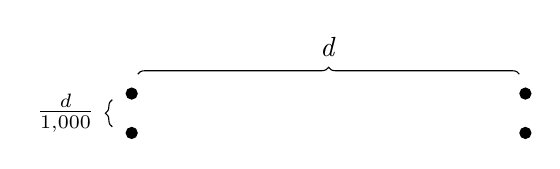
\begin{tikzpicture}[auto, node distance = 3cm, main node/.style={dot}]
\node[circle, draw, fill=black,
                        inner sep=0pt, minimum width=4pt](1) at (0,0) {};
\node[circle, draw, fill=black,
                        inner sep=0pt, minimum width=4pt](2) at (5,0) {};
\node[circle, draw, fill=black,
                        inner sep=0pt, minimum width=4pt](3) at (0,-.5) {};
\node[circle, draw, fill=black,
                        inner sep=0pt, minimum width=4pt](4) at (5,-.5) {};
\draw[decoration={brace,raise=7pt},decorate] (1) -- (2) node[midway, above = 10pt] {\textit{d}};
\draw[decoration={brace, mirror, raise = 7pt},decorate] (1) -- (3) node[midway, left = 10pt] {\textit{$\frac{d}{1,000}$}};
% \draw (2) -- (4);
% \draw (3) -- (4);
\end{tikzpicture}\]\\
\vspace{.5cm}
As we increase $d$, we would expect this to have 1 cluster, then 2, then 4.
}
\frame{\frametitle{Magnitude Example}
Plot of magnitude as we ``zoom in" on the space:
\centerline{
\includegraphics[width = 1.2\textwidth]{../Figures/4_point.png}
}
}
\section{}

\frame{
\huge
\begin{center}Thank you! \end{center}
\vspace{1cm}
\[
\includegraphics[width=.5\textwidth]{../Figures/mobius_strip.png}
\]
}
\frame{\frametitle{Sources}
\tiny
\nocite{*}
\bibliographystyle{abbrv}
\bibliography{../Drafts/bibliography.bib}
}

\end{document}

